\chapter{\ifenglish Background Knowledge and Theory\else ทฤษฎีที่เกี่ยวข้อง\fi}

เนื้อหาในบทนี้ จะกล่าวถึงหลักการที่นำมาประยุกต์ใช้ในการพัฒนาระบบของ Flowy และ Flowider

\section{Web Development}
\subsection{MVC}
MVC หรือ Model-View-Controller~\cite{concept_mvc} คือแบบแผนโครงสร้างทางซอฟต์แวร์ (software architectural pattern) ในการพัฒนาโปรแกรม โดยมีการแบ่งแยกสัดส่วนการทำงานชัดเจนระหว่าง User Interface, Controller หรือ Business Logic และ Database (Model) ซึ่งกลไกการทำงานนั้นผู้ใช้งานจะกระทำ (interact) ผ่าน user interface เพื่อทำการส่ง request ไปยัง controller ให้ทำกระทำการ (manipulate) กับฐานข้อมูลอีกทีหนึ่งเพื่อส่งกลับมาเป็น response ผ่าน controller แล้วนำมาแสดงผลผ่าน user interface อีกครั้ง
\begin{figure}[h]
  \begin{center}
  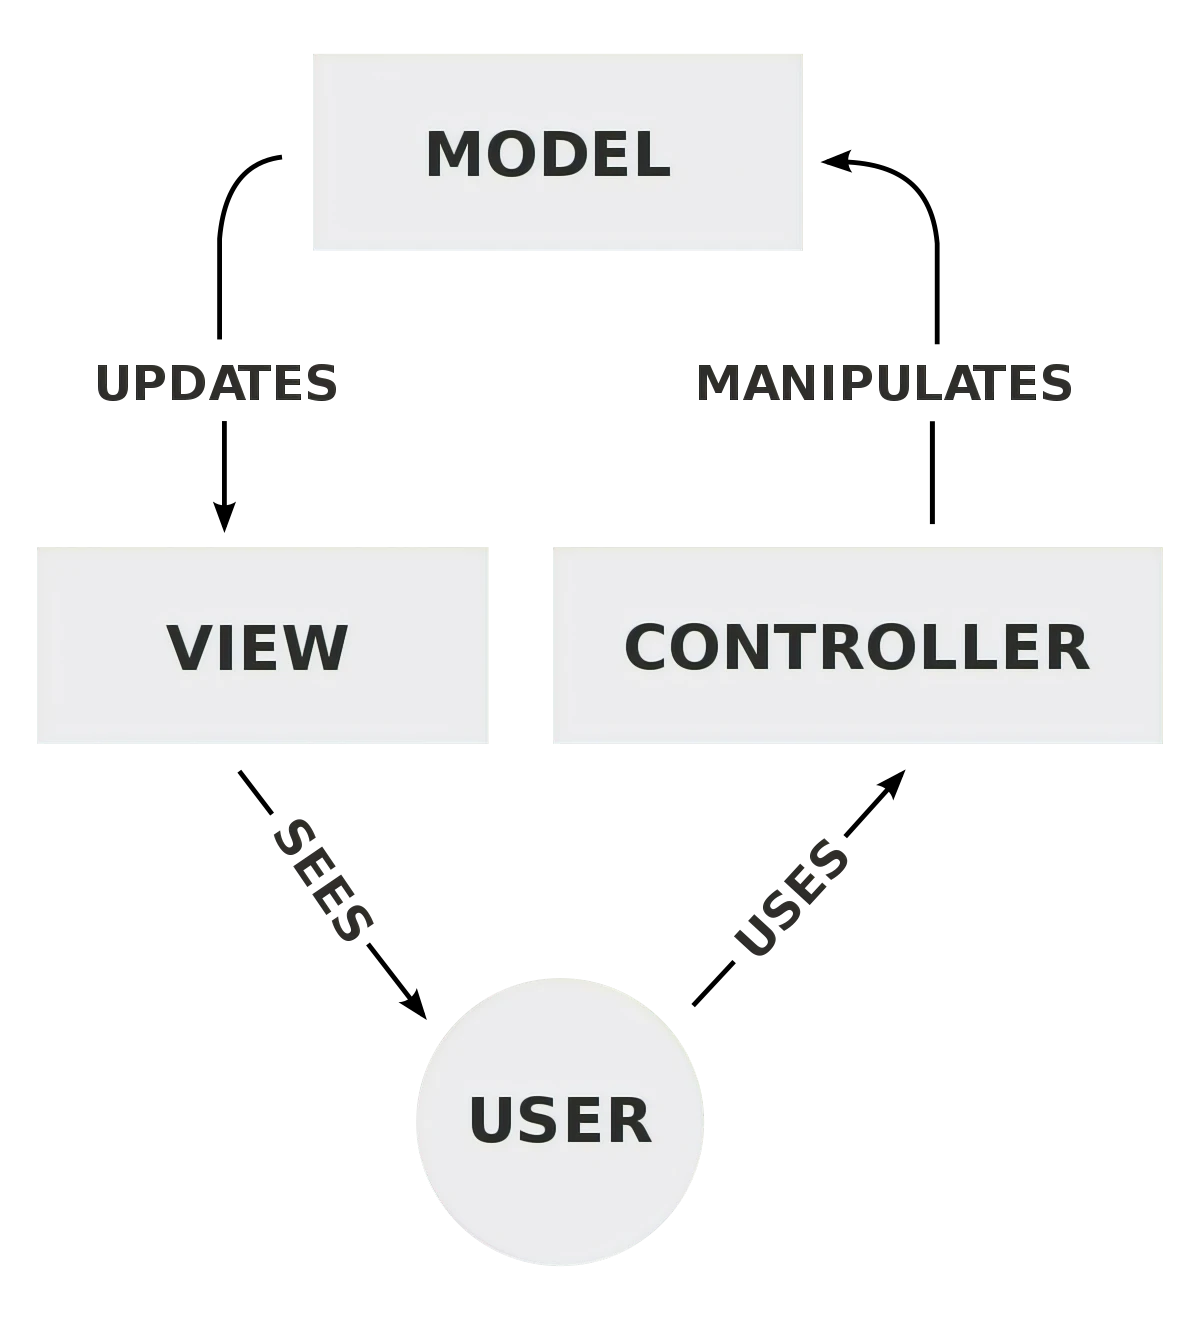
\includegraphics[width=2.5in]{./image/MVC.png}
  \end{center}
  \caption[MVC]{แผนผัง MVC หรือ Model-View-Controller~\cite{mvc}}
  \label{fig:MVC}
\end{figure}

\subsection{REST API}
REST API หรือ Representational State Transfer เป็นรูปแบบหนึ่งของ API (Application Programming Interface) ที่ทำการส่ง request และ response ผ่าน HTTP methods เช่น \textit{\texttt{Get}, \texttt{POST}, \texttt{PUT}, \texttt{DELETE}} เป็นต้น ผ่าน URL ของ API ที่ถูกออกแบบจัดสรรให้ทำหน้าที่ที่เฉพาะเจาะจงไว้เรียบร้อยแล้ว โดยเรียกได้อีกชื่อหนึ่งว่า \textbf{API Endpoints}

ซึ่งอุปกรณ์ของ client จำเป็นต้องส่ง request ไปยัง server ตาม endpoint ที่ถูกกำหนดหน้าที่การทำงานไว้แล้ว จากนั้น server จึงจะส่ง response กลับมาในรูปแบบใด ๆ ก็ได้ ซึ่งรูปแบบที่เป็นที่นิยมคือรูปแบบของ JSON

\begin{itemize}
  \item ข้อดีของ REST API มีดังนี้~\cite{rest_vs_soap}
  \begin{itemize}
    \item ทำงานอยู่บนมาตรฐานของ HTTP method
    \item รูปแบบของ response มีหลายรูปแบบเช่น JSON, XML เป็นต้น
    \item รองรับการขยายระบบได้ง่าย/มีความ independent สูง เพียงแค่ client เชื่อมต่อกับ endpoint ก็พอ
    \item รองรับการทำ caching โดยอาศัยหลักการของ API gateway
    \item เข้ากันกับรูปแบบการพัฒนาแบบ MVC เป็นอย่างดี
  \end{itemize}
  \item ข้อเสียของ REST API มีดังนี้
  \begin{itemize}
    \item ไม่มีการสนับสนุนเรื่อง security มาตั้งแต่ต้น เราจำเป็นต้อง implement เอง
    \item การทำ limitation ต่าง ๆ ของ request size, response size จำเป็นที่จะต้องออกแบบเองตั้งแต่ต้น
  \end{itemize}
\end{itemize}

\subsection{Cloud Based Development}
Cloud Based Development~\cite{cloud_dev} คือการพัฒนาโปรแกรมโดยอาศัย service ต่าง ๆ จากผู้ให้บริการ cloud (Cloud Provider) เพื่อลดค่าใช้จ่ายต่าง ๆ ที่จะเกิดจากการ host โปรแกรมของตนเอง เพราะการ host โปรแกรมหรือบริการของต้นเองนั้นใช้ต้นทุนสูงในการซื้อ hardware อีกทั้งยังตามมาด้วยค่าใช้จ่ายในการซ่อมบำรุงหรือขยาย service ของตนเอง ในปัจจุบัน Cloud Based Development จึงเป็นที่นิยมเพราะไม่ต้องจัดการปัญหาเหล่านั้นด้วยตนเองและง่ายต่อการ deploy อีกด้วย

ตัวอย่าง Cloud Provider ในปัจจุบัน เช่น Amazon Web Service (AWS), Google Cloud Platform (GCP), Google Firebase, Microsoft Azure เป็นต้น

\subsection{Component-driven Development}
Component-driven Development (CDD)~\cite{cdd} คือรูปแบบการพัฒนาโปรแกรมที่มีลักษณะพิเศษและสอดรับกับการพัฒนาด้วย React.js (ซึ่งเป็นเครื่องมือที่เราใช้ในโครงงานนี้) เป็นอย่างดี ด้วยการมองภาพส่วนของโปรแกรมต่าง ๆ เป็น component เพื่อความสะดวกและรวดเร็วในการพัฒนาและความเป็นระเบียบตาม design pattern แบบ command pattern
\begin{itemize}
  \item ประโยชน์ของ Component-driven Development
  \begin{itemize}
    \item ทำให้การทำงานกับนักออกแบบง่ายขึ้น เนื่องจากนักออกแบบจะเริ่มการออกแบบจาก design system ก่อน ซึ่งมีรูปแบบเป็น component-driven อยู่แล้ว
    \item สามารถแบ่งความรับผิดชอบภายในทีมได้ง่าย เช่น คนหนึ่งรับผิดชอบ component หนึ่งไปเลย เป็นต้น
    \item สามารถนำ component ต่าง ๆ กลับมาใช้ซ้ำ (reuse) ได้
  \end{itemize}
\end{itemize}

\section{User Interface}
\subsection{Progressive Web Application (PWA)}
Progressive web application (PWA)~\cite{pwa} คือการทําเว็บไซต์ธรรมดา ให้ใกล้เคียงกับแอปพลิเคชั่นที่ดาวน์โหลดลงเครื่องมากที่สุด ทั้งในแง่รูปลักษณ์ ความเร็ว ไปจนถึงการใช้งาน รวมถึงมีการปรับการแสดงผล
ให้เหมาะกับอุปกรณ์ที่ใช้ เช่น smartphone, tablet และ desktop

ลักษณะที่สําคัญที่สุดของ progressive web application แบ่งออกได้เป็นดังนี้ \\
\textbf{Reliable:} มีความน่าเชื่อถือ สามารถใช้งานได้ตลอดแม้ว่าการทํางานของเครือข่ายจะไม่เสถียร \\
\textbf{Fast:} ต้องเร็ว ไม่ว่าจะมีอนิเมชั่นสวยหรือสิ่งใดก็แล้วแต่ การตอบสนองต่อผู้ใช้สําคัญที่สุด \\
\textbf{Engaging:} ผู้ใช้สามารถใช้งานมันไม่ต่างกับแอปพลิเคชั่นปกติ

\begin{itemize}
  \item ข้อดีของ progressive web application มีดังนี้
  \begin{itemize}
    \item ลด learning curve ในการเรียนรู้เครื่องมือใหม่เพื่อที่จะพัฒนา mobile native application ทำให้ประหยัดเวลาในการพัฒนาและสามารถเอาเวลาที่ลดได้ไปโฟกัสในเรื่องอื่น ๆ เช่น การพิสูจน์ความต้องการของลูกค้าหรือตลาด เป็นต้น
  \end{itemize}
  \item ข้อเสียของ progressive web applications มีดังนี้~\cite{bad_pwa}
  \begin{itemize}
    \item การเข้าถึงในส่วนของ hardware เช่น กล้องถ่ายภาพ, geolocation, NFC, Bluetooth เป็นไปได้ยากและไม่มีการจดจำการอนุญาตเข้าถึง ทำให้ผู้ใช้งานจำเป็นที่จะต้องกดยินยอมในบางครั้ง
  \end{itemize}

\end{itemize}

\subsection{Responsive Web Design}
Responsive web design~\cite{responsive} เป็นเทคนิคการออกแบบเว็บไซต์ซึ่งจะมีการคํานึงถึงการปรับเปลี่ยนขนาดของเว็บไซต์ให้เหมาะสมกับการแสดงผลบนหน้าจอขนาดต่าง ๆ และความละเอียดของหน้าจอในอุปกรณ์ที่
แตกต่างกัน เช่น คอมพิวเตอร์ โน้ตบุ๊ค โทรศัพท์มือถือ แท็บเล็ต เป็นต้น เพื่อให้ประสบการณ์การใช้งานของ user ดีมากยิ่งขึ้น
\begin{itemize}
  \item ข้อดีของ responsive web design แบ่งออกได้เป็นดังนี้
  \begin{itemize}
    \item ทําให้เว็บไซต์รองรับอุปกรณ์มือถือไปในตัว (mobile-friendly) ซึ่งปั จจุบันจํานวนผู้ใช้งานเว็บไซต์จากโทรศัพท์มือถือนั้นกําลังเพิ่มมากขึ้น
    \item ผู้ใช้สามารถใช้งานเว็บไซต์ได้ง่าย (user-friendly) ไม่ว่าจะเปิดเว็บไซต์ด้วยอุปกรณ์หรือขนาดหน้าจอใด ๆ ก็ตาม
    \item สนับสนุนการทํา search engine optimization (SEO) กับ Google ทั้งเวอร์ชั่น desktop และ mobile ในเว็บไซต์เดียว
  \end{itemize}
  \item ข้อเสียของ responsive web design แบ่งออกได้เป็นดังนี้~\cite{bad_responsive}
  \begin{itemize}
    \item การใช้เขียน code รูปแบบเดียวเพื่อรองรับหลายอุปกรณ์ อาจทําให้เกิดปัญหาตามมาได้ ตัวอย่างเช่น ในโทรศัพท์มือถือที่มีหน้าจอขนาดเล็ก การซ่อนเนื้อหาที่ไม่จําเป็น เช่น โฆษณา ในบางเว็บบราวเซอร์จะยังทําการโหลดข้อมูลเหล่านี้เข้ามาแสดงอยู่
    \item Image resizing ที่ไม่ได้ลดขนาดของตัวรูปภาพ แต่ใช้วิธีการย่อขนาดขณะแสดงผลเท่านั้น ซึ่งอาจทําให้โทรศัพท์มือถือต้องโหลดรูปเดียวกับที่แสดงบน desktop จึงทําให้เราเสียเวลาโดยไม่จําเป็น
  \end{itemize}
\end{itemize}

\section{Best Practices}
\subsection{Timezone Complexity}
เมื่อมีการกระทำกับ attribute ของ record ใด ๆ ที่มี data type ในรูปแบบ \textit{\texttt{TIMESTAMP}} ทาง RDBMS จะทำการเก็บข้อมูลใน attribute นั้นใน format date-time แบบ UTC โดย default ซึ่งเมื่อเราจะใช้งานใน timezone อื่น ๆ ที่ไม่ใช่ UTC (เช่น GMT+0700 เป็นต้น) จะมีปัญหาในการ query ในแต่ละครั้งที่จะได้ผลลัพธ์ไม่ตรงกับ timezone ที่ client ใช้งานอยู่

\subsubsection{Best Practice}
TIMESTAMP ที่เก็บในฐานข้อมูลจะยังเป็น UTC format เหมือนเดิม แต่ทุกครั้งที่ query จะทำการ convert เป็น GMT ใด ๆ ก็ตามที่ client ได้ทำการ request มาทุกครั้งก่อนจะส่ง response กลับไป กล่าวคือ จากการแปลงตั้งแต่ต้นทางก่อนที่จะบันทึกเข้ามาในฐานะข้อมูล เราทำการแปลงก่อนจะส่ง response กลับไป เพื่อที่จะได้ง่ายต่อการทำงานเมื่อใช้งานจากต่างประเทศ

\subsection{Image Collection as Pool}
เมื่อเราต้องทำงานกับรูปภาพที่จะทำการบันทึกเข้ามายังฐานข้อมูล ความจริงแล้วมีวิธีการทำงานกับรูปภาพหลากหลายมาก เช่น การแปลงเป็น Base64 URL, การเก็บเป็น BLOB เป็นต้น แต่วิธีที่เป็นที่นิยมสำหรับการพัฒนาแบบ Cloud Based Development เป็นดังวิธีการดังนี้

\subsubsection{Best Practice}
เราจะทำการอัพโหลดรูปภาพหรือไฟล์ที่ต้องการขึ้นไปยัง cloud provider ที่เราเป็นสมาชิกเอาไว้ จากนั้นนำ URL ที่ได้หลังจากการอัพโหลดแล้วมาบันทึกในตาราง relation table ที่มี unique ID ของแต่ละ entity เอาไว้ เพื่อง่ายและสะดวกต่อการเรียกใช้หรือ CRUD ต่อไป

\subsection{JSX Coding Style Guide}
เป็นธรรมดาที่ว่าการเขียนโปรแกรมของแต่ละคนนั้นมีสไตล์การเขียนโค้ดหรือ convention~\cite{convention} ที่ต่างกัน ซึ่งมันจะไม่เป็นปัญหาหากเราทำงานเพียงคนเดียว แต่ในความเป็นจริงนั้นเราต้องทำงานกับทีมที่เกี่ยวข้องเราจึงต้องมี \textit{กฏหรือธรรมเนียมปฏิบัติในการเขียนโค้ด} เพื่อให้การทำงานเป็นทีมนั้นสะดวกและเป็นแบบแผนเดียวกันมากขึ้น

\subsubsection{Best Practice}
เราใช้ระเบียบแบบแผนของ Airbnb (Airbnb JSX Style Guide)~\cite{airbnb_jsx} เป็นข้อตกลงร่วมกันระหว่างคนในทีม ในการกำหนดสไตล์การเขียนโค้ดสำหรับโครงงานนี้

\section{ความรู้ตามหลักสูตรซึ่งถูกนำมาใช้หรือบูรณาการในโครงงาน}
\subsection{Usability Heuristic Evaluation}
\textit{จากวิชา 269462 Intro to Human-Computer Interaction} \\
หลักการทั้ง 10 ข้อเพื่อเป็น guideline สำหรับการออกแบบ User Interface ให้มี usability ที่ดีและเป็นเกณฑ์ตรวจสอบ UI คร่าว ๆ ว่า UI มีปัญหา usability ด้านไหน (Effectiveness/Efficiency/Satisfaction) โดยกระบวนการประเมิณผลโดยใช้หลักการนี้เรียกว่า ''Usability Heuristic Evaluation''

\subsection{Relational Database}
\textit{จากวิชา 261342 Fundamental of Database Systems และ 261343 Database Systems Laboratory} \\
ความรู้เกี่ยวกับการออกแบบฐานข้อมูล การสร้างแผนผัง Unified Modeling Language (UML) และ ER diagram

\subsection{Object-Oriented Programming}
\textit{จากวิชา 261200 Object-Oriented Programming} \\
ความรู้เกี่ยวกับการเขียนโปรแกรมเชิงวัตถุ ซึ่งเป็นแนวคิดในการพัฒนาซอฟแวร์ที่เป็นที่นิยมในปัจจุบัน โดยเฉพาะอย่างยิ่งรูปแบบการพัฒนาแบบ MVC

\subsection{Scrum}
\textit{จากวิชา 261361 Software Engineering} \\
ความรู้เกี่ยวกับการทำงานแบบ Scrum ที่มีความคล่องตัวสูงและเน้นผู้ใช้งานเป็นศูนย์กลาง (user-centric) โดยอาศัยการพัฒนาเป็นรอบ (sprint) เพื่อนำผลิตภัณฑ์ในแต่ละ sprint ออกไปทดสอบกับผู้ใช้งานหรือลูกค้าเพื่อในมาปรับแก้ให้สอดรับตามความต้องการ (requirement) ของผู้ใช้งานให้ได้มากที่สุด

\section{ความรู้นอกหลักสูตรซึ่งถูกนำมาใช้หรือบูรณาการในโครงงาน}
\subsection{Design Thinking}
เป็นกระบวนการตั้งแต่ก่อนการสร้างผลิตภัณฑ์ใด ๆ ไปจนถึงการนำผลิตภัณฑ์ไปทดสอบกับกลุ่มลูกค้าหรือผู้ที่ประสบปัญหานั้น ๆ ที่เราจะต้องการแก้ปัญหาให้ โดยผ่าน 5 ขั้นตอนสำคัญได้แก่ Empathize (การทำความเข้าอกเข้าใจปัญหา), Define (กำหนดปัญหาที่ต้องการจะแก้ไข), Ideate (ระดมไอเดียวิธีการแก้ไขปัญหา), Prototype (ทำตัวต้นแบบเพื่อนำไปทดสอบ), Test (ทดสอบเพื่อดูว่าไอเดียที่คิดสามารถแก้ไขปัญหาได้จริง)

\subsection{Problem-Solution Fit}
เป็นกระบวนการคิดแบบธุรกิจ startup ที่ต่อยอดมาจากกระบวนการ design thinking โดยก่อนที่จะดำเนินธุรกิจใด ๆ เราจำเป็นที่จะต้องให้ผลิตภัณฑ์ของเราตอบโจทย์ความต้องการของลูกค้าได้อย่างแท้จริงก่อน จึงจะสามารถดำเนินแผนธุรกิจอื่น ๆ เช่น การเก็บค่าบริการ, การขยายธุรกิจ ฯลฯ ต่อไปได้

\subsection{Business Model Canvas}
ตาราง 9 ช่องสำหรับการใส่รายละเอียดสำคัญก่อนเริ่มทำธุรกิจเพื่อเห็นภาพทั้งหมดก่อนว่าลักษณะธุรกิจของเราเป็นอะไร, ทำอะไร, เพื่อใคร รวมถึงกิจกรรมหลักทางธุรกิจต่าง ๆ, ต้นทุน, ช่องทางรายได้ที่จะได้รับด้วยเช่นกัน